\documentclass[american,titlepage,oneside]{ntnuthesis}

\title{An NTNU Thesis \LaTeX{} Document Class}
\shorttitle{An NTNU Thesis Document Class}
\author{Community of Practice in Computer Science Education at NTNU}
\shortauthor{CoPCSE$@$NTNU}
\date{CC-BY \ntnuthesisdate}

\addbibresource{thesis.bib}


% From https://www.overleaf.com/learn/latex/Glossaries

\makeglossaries % Prepare for adding glossary entries


\newglossaryentry{latex}{
        name=latex,
        description={Is a mark up language specially suited for
scientific documents}
}

\newglossaryentry{bibliography}{
    name=bibliography,
    plural=bibliographies,
    description={A list of the books referred to in a scholarly work, typically printed as an appendix}
}

\newglossaryentry{maths}{
    name=mathematics,
    description={Mathematics is what mathematicians do}
}

\newglossaryentry{locode}{
    name=UN/LOCODE,
    description={Five-letter geographic coding scheme maintained by the UN. The codes are assigned to, among others, ports where the first to letters represents a country code and the remaining three represents a location}
}

\newglossaryentry{aivdm}{
    name=AIVDM/AIVDO,
    description={The protocol used by AIS messages where AIVDM contains data received from other vessels, and AIVDO contains data from the owner vessel}
}


% --------------------
% ----- Acronyms -----
% --------------------

\newacronym{phd}{PhD}{philosophiae doctor}
\newacronym{CoPCSE}{CoPCSE@NTNU}{Community of Practice in Computer ScienceEducation at NTNU}
\newacronym{gcd}{GCD}{Greatest Common Divisor}
\newacronym{mo}{MO}{Maritime Optima AS}
\newacronym{ais}{AIS}{Automatic Identification Systems}
\newacronym{gis}{GIS}{Geographical Information System}
\newacronym{imo}{IMO}{International Maritime Organization}
\newacronym{mmsi}{MMSI}{Maritime Mobile Service Identity}
\newacronym{ntnu}{NTNU}{Norwegian University of Technology and Science}
\newacronym{ml}{ML}{Machine learning}
\newacronym{gt}{GT}{Gross Tonnage}
\newacronym{cog}{COG}{Course Over Ground}
\newacronym{sog}{SOG}{Speed Over Ground}
\newacronym{rot}{ROT}{Rate of Turn}
\newacronym{eta}{ETA}{Estimated Time of Arrival}
\newacronym{sspd}{SSPD}{Symmetric Segment-Path Distance}
\newacronym{dbscan}{DBSCAN}{Density-based spatial clustering of applications with noise}
\newacronym{rf}{RF}{Random Forest}
\newacronym{knn}{k-NN}{k-Nearest Neighbor}
\newacronym{rnn}{RNN}{Recurrent Neural Network}
\newacronym{svm}{SVM}{Support Vector Machine}
 % add glossary and acronym lists before document

\begin{document}

\chapter*{Abstract}

This thesis develops a new approach for automating the cost impact of security incidents. The method is based on detecting security incidents in news articles and then using an event study to determine the change in stock price resulting from the security incident. The main finding is that TODO.
\chapter*{Sammendrag}

TODO

\tableofcontents
\listoffigures
\listoftables
\lstlistoflistings

\printglossary[type=\acronymtype] % Print acronyms
\printglossary                    % Print glossary

\newcommand{\paragraphheader}[1]{\paragraph{#1}\mbox{}\\}
\newcommand{\todo}[1]{{\color{olive}\textbf{TODO:}\color{olive}#1}} % items to do

\setlength{\parindent}{4em}
%\setlength{\parskip}{1em}

\chapter{Introduction}

Thesis introduction chapter test.

Test commit.

Over the years, several thesis templates for \LaTeX{} have been developed by different groups at NTNU\@. Typically, there have been local templates for given study programmes, or different templates for the different study levels – bachelor, master, and \acrshort{phd}.\footnote{see, e.g., \url{https://github.com/COPCSE-NTNU/bachelor-thesis-NTNU} and \url{https://github.com/COPCSE-NTNU/master-theses-NTNU}}

Based on this experience, the \acrfull{CoPCSE}\footnote{\url{https://www.ntnu.no/wiki/display/copcse/Community+of+Practice+in+Computer+Science+Education+Home}} is hereby offering a template that should in principle be applicable for theses at all study levels. It is closely based on the standard \LaTeX{} \texttt{report} document class as well as previous thesis templates. Since the central regulations for thesis design have been relaxed – at least for some of the historical university colleges now part of NTNU – the template has been simlified and put closer to the default \LaTeX{} look and feel.

The purpose of the present document is threefold. It should serve (i) as a description of the document class, (ii) as an example of how to use it, and (iii) as a thesis template.

\chapter{Related work}

The topic of \acrfull{ais} -based predictions has already been explored quite extensively, especially in recent years as \acrshort{ais} systems has become an enforced standard for commercial vessels in the industry. However, the \acrshort{ais} standard has mainly been standardized for the purpose of maritime safety and navigation, and the existing academic work on this topic reflects this. Therefore, most of the related work consists of vessel trajectory predictions for the purpose of foreseeing a future collision situation or for detecting anomalies from detected shipping lanes. These types of predictions are applicable for predicting a vessel's future position in a short time interval, in a smaller geographical scale, but with high positional accuracy.

In order to establish the current state of the art of the topic area and establish to what extent the literature answers the proposed research questions, a literature review was conducted which is explained in this section.

\section{Literature review}
\label{sec:lit_review}

As already mentioned, based on initial research into the thesis' topic area, there seemed to be an apparent trend in motivations of related work directed at short-term predictions for safety and navigational purposes. In contrast, this thesis aims at using \acrshort{ais}, and other attributes, for longer term predictions, or more accurately, port destination predictions. However, because of the exploratory nature of thesis, the literature review conducted was broad in order to include work that might have taken a different approach to solve the same problem. In order to organize the resulting papers, a categorical separation of papers based on motivation was defined as follows:

\begin{enumerate}
\setcounter{enumi}{-1}
    \item The paper's motivation deems it completely irrelevant to the topic area.
    \item The paper's motivation includes vessel predictions, but on a smaller time or geographical scale making it irrelevant for comparison.
    \item The paper's motivation includes destination predictions making it relevant enough for further analysis.
\end{enumerate}

\textit{Category 0} is defined to filter out papers that were irrelevant but could not be excluded by narrowing the search query. \textit{Category 1} includes paper that relates to the established trend mentioned earlier where the proposed method seems relevant on a small scale, but is ultimately not applicable to the thesis' problem area. It also includes papers that considers relevant topics but not relevant solutions. Finally, the papers labeled with relevancy \texttt{2} falls within \textit{Category 2} and includes papers that falls within the same topic area and are relevant for further analysis in regards to the research questions.

In order to determine what papers fitted \textit{category 1} and \textit{2}, papers with a relevance higher than zero were further analyzed in order to determine the following attributes:

\begin{itemize}
    \item Motivation and goals
    \item Data source
    \item Prediction method
    \item Geographical extent
    \item Time interval
    \item Validation method
    \item Validation, or performance metrics
\end{itemize}

In this literature review, the primary search engine used was \textit{Scopus}\footnote{\url{https://www.scopus.com/}} as it seemed to return the best search results without an excess of less relevant papers that was returned by other search engines such as \textit{ScienceDirect}\footnote{\url{https://sciencedirect.com}} and \textit{Google Scholar}\footnote{\url{https://scholar.google.com}}. Furthermore, the chosen search query was also ran on the \acrshort{ntnu} university library \textit{Oria}\footnote{\url{http://ntnu.oria.no/}} in order to find overlap and additional results not found by \textit{Scopus}.

\subsubsection{Search query and filters}

The objective of the literature review was to conduct a broad search detecting papers related to multiple relevant topics such as \textit{vessel destination prediction}, \textit{vessel trajectory prediction}, \textit{vessel availability forecasting}, and \textit{maritime logistics}. Therefore, the search query used in the literature review was designed to find papers within multiple topics and was derived at from testing multiple queries on multiple search engines.

For instance, the following queries were tested using the search engine provided by \textit{ScienceDirect}:

\begin{itemize}
    \item `vessel trajectory' OR `ship trajectory' resulted in \textbf{421} papers
    \item ais AND (`vessel trajectory' OR `ship trajectory') resulted in \textbf{150} papers
    \item ais AND (prediction OR predicting) AND (`vessel trajectory' OR `ship trajectory') resulted in \textbf{108} papers
\end{itemize}

The above queries returned a large number of papers relevant to \textit{category 1}, so in order to find more relevant papers, more specific queries were also tested:

\begin{itemize}
    \item `vessel destination' OR `ship destination' OR `vessel availability' resulted in \textbf{389} papers
    \item ais AND (`vessel destination' OR `vessel availability') resulted in \textbf{25} papers.
    \item ais AND (predicting OR forecasting) AND (`vessel destination' OR `vessel availability' OR `ship supply') resulted in \textbf{18} papers.
\end{itemize}

The search terms that seemed to return the most relevant papers was combined into the final query used in the literature review shown in \cref{lst:search_query}.

\begin{lstlisting}[
    caption={Search query used in literature review},
    label=lst:search_query
]
ais AND (
    predict OR predicting OR forecast OR forecasting
) AND (
    vessel OR ship OR maritime
) AND (
    destination OR availability OR supply OR trajectory OR logistics
)
\end{lstlisting}

Moreover, the following filters was used to limit the search result:

\begin{itemize}
    \item The paper must be published in the last 5 years.
    \item The paper must be available in English.
    \item The paper must be available using the access rights provided by \acrshort{ntnu}.
\end{itemize}

As already mentioned, the search query was ran on the search engine \textit{Scopus}, thus the search query and filters was modified to the search engine's format as shown in \cref{lst:search_query_scopus}.

\begin{lstlisting}[
    caption={Search query used in Scopus including filters},
    label=lst:search_query_scopus
]
TITLE-ABS-KEY (
    ais AND (
        prediction OR predicting OR forecast OR forecasting
    ) AND (
        vessel OR ship OR maritime
    ) AND (
        destination OR availability OR supply OR trajectory OR logistics
    )
) AND PUBYEAR > 2014 AND (
    LIMIT-TO ( DOCTYPE , "cp" ) OR
    LIMIT-TO ( DOCTYPE , "ar" ) OR
    LIMIT-TO ( DOCTYPE , "re" ) OR
    LIMIT-TO ( DOCTYPE , "ch" ) OR
    LIMIT-TO ( DOCTYPE , "Undefined" )
) AND ( EXCLUDE ( SUBJAREA , "MEDI" ) )
\end{lstlisting}

\subsubsection{Results}

The defined search query returned a total of \textbf{80} papers from the \textit{Scopus} search library and \textbf{22} from \textit{Oria} where out of which \textbf{7} papers did not overlap with results from \textit{Scopus}. These \textbf{87} papers formed the basis of the literature review.

The papers were evaluated based on the level of relevance as defined in \cref{sec:lit_review}. Out of the \textbf{80} papers, \textbf{49} fell within \textit{category 0}, \textbf{32} within \textit{category 1}, and \textbf{6} within \textit{category 2}.

The large number of irrelevant papers resulted from the broadness of the query that was designed to find results in multiple topic areas. Furthermore, there were some papers that was medical in nature but not labeled correctly in \textit{Scopus} and was returned as the term \acrshort{ais} is also an acronym of \textit{Arterial Ischemic Stroke}. Some papers were also not publicly available but was not excluded by the search, while other papers were deemed irrelevant as they concerned topics such as mapping fishing areas in a specific region, power and performance predictions using \acrshort{ais} data, or high level discussions of potential applications of \acrshort{ais} data analysis.

The large number of papers within \textit{category 1} further confirms the general trend of \acrshort{ais} -based predictions as the primary goal of most of the resulting papers were to predict future positions of vessels within a shorter time intervals for the purpose of either safety and navigation or anomaly detection. None of the papers within \textit{category 1} seemed applicable to predict vessel destination ports at a global scale, however, for reproducibility, all papers with a relevancy of \textit{1} are listed in \todo{APPENDIX}.

% most relevant papers collected from literature review
\begin{table}[tbp]
    \centering
    \csvreader[
      tabular=p{0.55in} p{1.7in} p{1.6in} p{0.7in} p{0.3in},
      table head=\hline \bfseries{Paper} & \bfseries{Goal} & \bfseries{Pred. method} & \bfseries{Geo-extent} & \bfseries{Time},
      before line=\\\hline,
      late after last line=\\\hline % horizontal line at the end of the table
    ]{
        csvtables/most_relevant.csv
    }{}{\csvlinetotablerow}
\caption{Papers collected from literature review with relevant geographical and time limitations}\label{tab:most_relevant_papers}
\end{table}

The remaining \textbf{}6 papers (listed in \cref{tab:most_relevant_papers}) were deemed relevant enough to further analyze in order to answer the research questions defined in \cref{sec:research_questions}. In addition, \cite{lechtenberg2019}, which was discovered during the process of testing queries, was also included in the analysis as it seemed highly relevant toward availability forecasting, but did not appear when using the two search engines in the final review.


\todo{copied from RPP}
\paragraphheader{RQ 1: What prediction methods can be used to predict vessel availability?}

\cite{lechtenberg2019} used a combination of several prediction methods in order to predict vessels’ next destination region, estimated time of arrival (ETA), and anchor time (AT) within regions. For predicting the next destination region the \textit{Markov Decision Process} was used as there are a limited number of possible regions (44) that a vessel can travel to. For the ETA and AT predictions, an \textit{XGBoost} method was applied. However, the extent of the regions was not disclosed, and although it was explained that port frequencies were used to determine regional availability, the accuracy of port frequencies was also not disclosed.

\paragraphheader{RQ 2: What prediction methods can be used to predict vessel destinations?}

\cite{ZHANG2020102729} was the second paper found which fitted within \textit{category 1}, and used a random forest approach to compare a given vessel’s current trajectory with all historical trajectories from the same departure port. They also used port frequency to normalize the results. In this way, they managed to achieve good results by combining both methods for predicting port destinations as well as city destinations. This method was unique as it considers multiple aspects of vessel voyages compared to the other methods.\\

\paragraphheader{RQ 2A: What type of data did they rely on?}

All of the aforementioned methods relied on historical AIS data collected by a combination of satellite and land-based base stations. \cite{ZHANG2020102729} also relied on an extensive port data base consisting of over \textbf{10 000} ports.

\paragraphheader{RQ 2B: How much depth of the data was relevant to the results?}

\cite{ZHANG2020102729} exclusively relied on the navigational data supplied by the AIS protocol. The navigational part of the AIS protocol includes coordinates, speed over ground (SOG), rate of turn (ROT), course over ground (COG), and more. Furthermore, \cite{ZHANG2020102729} also considered port frequencies, however, this frequency is deducted from the navigational part of the AIS data. Similarly, \cite{lechtenberg2019} also used port frequencies to predict regional availability, ETA, and AT. As already mentioned in \cref{sec:problem_desc}, destination and ETA values are included in the AIS protocol, however, as they are manually inputted by crew members they are not accurate. This is reflected in the existing literature as none of the aforementioned methods takes these values into consideration. Thus, it seems that all the relevant research ultimately only considers the navigational part of the AIS protocol for future predictions.

\paragraphheader{RQ 2C: How successful were they at predicting vessel destinations?}

\cite{lechtenberg2019} claims a \textit{98\%} accuracy when it comes to predicting a vessel’s next region, however, this value is presumed to vary depending on the size of the regions which is not disclosed in the paper. \cite{ZHANG2020102729} claims to have achieved a \textit{66.57\%} accuracy level for port-based predictions and \textit{81.65\%} accuracy for city-based predictions. As there is very little research that directly concerns predicting port or region destinations it is hard to establish a general accuracy of the state of the art. The closest assumption would be around \textit{70\%} for port predictions and \textit{98\%} for region predictions.

\paragraphheader{RQ 2D: How applicable were they toward predicting vessel availability?}

\cite{lechtenberg2019} was directly applicable and applied toward predicting vessel availability with a global set of regions. \cite{ZHANG2020102729} was not directly applied to forecast availability although it shows a very promising and generic method of predicting vessel’s future destinations unrestricted from time intervals or geographical areas. It is therefore very applicable toward predicting availability if applied to a global set of vessels. The rest of the aforementioned papers does not seem applicable toward availability if not combined with other methods that enable them to give accurate predictions globally.

\paragraphheader{RQ 3: How can the quality of the prediction methods be ensured?}

\cite{lechtenberg2019} does not go very in-depth on this topic, however, the paper mentions dividing the data into \textit{90\%} training data and \textit{10\%} test data. The accuracy metric is taken from how much of the test data was accurate. \cite{ZHANG2020102729} did an extensive evaluation of their method including the five-folder cross-validation method to ensure the model is not over-fitted. This process includes dividing the data into five “folders” and using one folder at a time for evaluation and the others for training. If the general accuracy does not vary much across the evaluation folders, the model is not overfitted.

\paragraphheader{RQ 3A: What metrics, or measurements, are used to establish quality?}

It seems that accuracy is the main measurement used to establish quality. Furthermore, \cite{lechtenberg2019} mentions using both the “mean absolute error” (MAE) and the “root mean square error” (RMSE) as quality indicators. \cite{ZHANG2020102729} mainly uses “average prediction distance error” (APDE) as their quality indicator which is based on the distance between the predicted trajectory and the actual trajectory.

\paragraphheader{RQ 4: How extensive is the impact of considering segmentation for prediction methods?}

None of the papers found within the research areas considers any type of segmentation of vessels. It is, therefore, impossible to answer this research question based on the current state of the art of the problem area.


\begin{sidewaystable}
    \centering
    {\small
    \begin{tabular}{|l|l|l|l|l|l|l|}
    \hline
        Paper & Motivation & Prediction method & Geographical scale & Time scale & Validation method & Validation metrics \\ \hline
        \cite{Alizadeh2020PredictionTrajectory} & trajectory similarity measurement for prediction of positions at time intervals & "spatial distance, bi-directional distance, speed distance" & "region (strait of georgia, USA)" & "10, 20, 30 minutes" & "sorenson similarity index (SSI), case study in region" & accuracy \\ \hline
        \cite{Alizadeh2021VesselData} & Vessel trajectory prediction for collision avoidance & "LSTM (RNN) with trajectory distance similarity measurements (TSSP, PSSP, TSSPL)" & "Strait of Georgia, USA" & Short term (10 - 40 mins) & 1 to 8 division of training and validation set & haversine distance accuracy (0.8 km to 3.5 km from 10-40 mins) \\ \hline
        \cite{Borkowski2017TheFusion} & data fusion prediction for collision avoidance integrated in navigation system & "ANN, data fusion, GRNN" & small (collision avoidance) & small & integrated and tested in real naviagtional system & RMSE \\ \hline
        \cite{Brandt2017MovingPrediction} & short time predictions of moving objects & "moving object data stream mangement systems, kNN " & "small, region in US" & small (10 minutes) & test cases & not explained \\ \hline
        \cite{Burger2020DiscretePrediction} & trajectory predictions for filling in gaps in AIS data & "DKF (discrete kalman filters), LRM" & small & small & single cases analysis on a vessel comparing two models & MED (mean euclidea distance) \\ \hline
        \cite{Chen2020ThePrediction} & cluster reconstruction not requiring training phase for short time frames & NPC clustering finding best possible next points & small & small & extensive comparisons with other methods & "accuracy, distance error" \\ \hline
        \cite{Dalsnes2018ThePrediction} & collision detection for autonomous vessels & NCDM & small (collision detection) & small (collision detection) & 90/10 training validation sets & RMSE \\ \hline
        \cite{Dijt2020TrajectoryShips} & collision avoidance for autonomous ships & sequence to sequence neural network & small (collision avoidance) & small (collision avoidance) & "90/10 data split of six hours trajectories, cross folder validation" & "absolute trajectory error, RMSE, MAE" \\ \hline
        \cite{DIng2020ALSTM} & longer time and multidimensional trajectory predictions & LSTM & small & 5-20 minutes & "training, validation, test set (8:1:1)" & MSE \\ \hline
        \cite{Forti2020PredictionNetworks} & sequence-to-sequence RNN approach & RNN with LSTM encoder-decoder architecture & region & small & 5-fold cross validation & RMSE \\ \hline
        \cite{Guo2018TrajectoryChain} & trajectory predictions MDTN (mobile delay tolerant network) & k-order multivariate markov chain & region (grid based) & small & "simulation, experiments" & accuracy \\ \hline
        \cite{Hexeberg2017AIS-basedPrediction} & collision detection & single neighbor search (SPNS) & region (trondheim) & small (10 minutes) & "training, validation sets, manually selected scenarios, validate with real trajectory" & RMSE \\ \hline
        \cite{Jin2020MaritimeNetwork} & longer range predictions for security motivations & "RNN, LSTM" & regional/small & small & model simulation & "distance accuracy over time, MAE, SSE" \\ \hline
        \cite{Kim2018PreprocessingArea} & predictions for Vessel Traffic Service (VTS) & NN & small & small & case study on region & speed and distance error \\ \hline
        \cite{Li2018ShipMining} & ceaner data extraction and mining for predictions & RBF neural network model & small (tested on river in china) & small-medium (hours) & simulation/case study on river in china & trajectory difference from real to simulated \\ \hline
        \cite{Li2019Long-termData} & longer term predictions for collision avoidance & "LSTM, longest comomon subsequence(LCS) algorithm, DBSCAN clustering" & small / collision avoidance & small / collision avoidance (15 min) & "applied to 4 regions, case studies" & distance error \\ \hline
        \cite{Lian2019ResearchAlgorithm} & "investigating particle filtering, near prediction, least squares estimation approach to predictions for smaller scale predictions" & "linear prediction, least squares, particle filtering" & small / collision avoidance & small / collision avoidance & "simulation, 9 hours of data" & "distance error, speed error" \\ \hline
        \cite{Liu2019VesselACDE-SVR} & trajectory prediction that also handles real time at sea & "SVR, ACDE, RNN" & small / collision avoidance & small / collision avoidance & training/validation sets & distance error \\ \hline
        \cite{Liu2020PredictingLearning} & "predicting trajectories for ship management, interpolating method for filling in missing AIS in trajectory" & "LSS-VM (least-squares support-vector machines) for predictions, cubic spline function to regulate trajectories via interpolation" & "independent of regions, but on a small scale (predicting distance not arrival ports)" & small (predicting next positions in trajectory) & four random trajectories selected for predictions & accuracy in distance/meters from actual trajectory \\ \hline
        \cite{Mao2018AnMining} & database for trajectory prediciton and mining & "interpolating trajectory reconstruction, are of interest bsed grid search, ELM and SLFN for predictions" & region based & medium (20 - 40 minutes) & original vs predicted trajectory & distance error \\ \hline
        \cite{Murray2018AOperations} & collision detection for autonomous vessels & Single point neighboir search method & small (collision detection) & 5-30 minutes & 90/10 training validation sets & RMSE \\ \hline
        \cite{Murray2019AnVessels} & collision avoidance & "gaussian mixture modelling, principle component analysis" & small / collision avoidance & small / collision avoidance & running 100 times randomly selecting points & distance error \\ \hline
        \cite{Murray2020AData} & trajectory predictions for early warnings and safety & "GMM clustering (gaussian mixture model), novel dual autoencoder" & region (tromsø) & 30 minutes (1 year or historical AIS) & distributed accuracy over time in the future (predicted positions vs actual positions) & accuracy at time intervals \\ \hline
        \cite{Rong2019ShipModel} & modelling uncertainty of trajectory predictions & "Bayesion model, Gaussian Process" & small / collision avoidance & "small / collision avoidance (10, 20, 30)" & "case study in region, training / validation data" & "accuracy, distance error" \\ \hline
        \cite{Suo2020ANetwork} & trajectory predictions for early warnings and safety & "GRU (gate recurrent unit), DBSCAN, comp. with LSTM" & tested on single port in china & "small, minutes to hour" & "training, validation, test set (not defined how much)" & accuracy \\ \hline
        \cite{Tafa2019AutomaticPrediction} & synthetic route representation and predictions & "DBSCAN, route similarity probability model" & east china sea region & 10-80 minutes & simulation & accuracy \\ \hline
        \cite{Tang2019ANetwork} & collision avoidance for automonous ships & LSTM & region in china & uses 10 min of data to predict 20 next minutes & training/validation sets & "MAE, MSE" \\ \hline
        \cite{Uney2019DataModels} & forecasting trajectories from historical and streaming trajectories & directed grid based bayesion model / gaussian mixture forecast density & tested on region (15x15 grid) & any (tested with 2 months of data) & real life case study in region & not explained \\ \hline
        \cite{Virjonen2018ShipMethod} & predictions in area in finnland that has to be several hours ahead in time & k-nearest neighbours & medium (region of finnland test case) & "medium, several hours" & nested leave-one-out-cross-validation (LOOCV) & distance accuracy \\ \hline
        \cite{Wang2020VesselGRU} & predicting vessel berthing trajectory for safety and collision avoidance & "Bi-GRU (tensorflow, keras)" & single port in china & small (minutes) & "training, validation set (not defined ratio), compared to other models" & MSE \\ \hline
        \cite{Xiao2020BigTechniques} & "for collision avoidance, better quering, more effective predictions" & "knowledge based particle filtering (PF), MLNN" & "smaller, limited to collision avoidance" & 3-10 minutes & testing different scnarios i.e. case studies & "sog, coc, and distance error" \\ \hline
        \cite{You2020ST-Seq2Seq:Prediction} & sequence-to-sequence RNN approach & "seq2se1 GRU, RNN, encoder/decoder" & "small, limited to 10m trajectories" & 10 minutes & "analysis in region (few rivers in china), training/validation set" & "AdaGrad, RMSProp" \\ \hline
        \cite{Zheng2020HeterogenousModeling} & combining multiple datasources like GPS and ARPA with AIS to improve predictions for safety & LSTM (on different data and a fusion component to merge the predictions) & small & small & "training, validation (1:10), and compare to other model" & MSE \\ \hline
        \cite{Zhou2019ShipNetwork} & collision avoidance in busy areas & back propagation nerual network & region (area in china) & small & training/validation 70/30 & RMSE \\ \hline
    \end{tabular}
    }
\end{sidewaystable}
\chapter{Choice of methods}

(copied from RPP, work from Mobile Spec. should be added here)

As the intended scope of the Master’s thesis consists of extending on an existing method of vessel predictions, the choice of methods mainly includes deciding on the most promising and expandable prediction method that is based on historical AIS data and shows a high level of accuracy. Next, the following phases are estimated to take place in the process: data evaluation, algorithm evaluation, algorithm improvements, and vessel availability pipeline.

\section{Choosing the most promising prediction method}

Further expanding on the expandability requirement, an important prerequisite is that it would be possible to apply Maritime Optima’s vessel segmentation to improve the model, thus the selected method would also have to support the possibility of labeling the dataset with additional information about the vessel. Another important prerequisite would be the possibility of applying the predicting method to a global set of vessels in order to forecast the vessel supply of availability. This could prove to be challenging in terms of setting up a scalable pipeline as well as making sure that the computation time is manageable either as a pre-computation step or on-demand computation of availability. However, for the scope of the thesis, only a prototype of the pipeline is expected to be completed.

Moreover, in the NTNU course called \textit{“IMT4889 - Specialization in mobile/wearable technologies”}, a similar, more specialized literature review was conducted by the author in order to provide a more in-depth analysis of the existing prediction methodologies. This literature was more specialized as it investigated existing prediction methods based on metrics such as relevance, performance, and development cost. The resulting report proposes prediction methods that show the most promise in regards to the evaluation criteria. The choice of methods is therefore based on two reviews of the current literature thoroughly analyzing the most prevalent prediction methods previously applied to similar problem areas. To summarize the findings of existing methods and the process of selecting prediction method:

The methods described in \cite{pallotta} seemed promising at predicting port destinations, however, only within a limited bounding area which had to include a substantial amount of systematic traffic. \cite{Daranda2016NeuralNA} described a method that could predict a trajectory of a vessel, but it did not seem applicable at predicting port destinations at a global scale. This assumption was also corroborated by \cite{ZHANG2020102729} in their analysis of related work: \textit{“[...] These works achieved promising prediction results on vessels’ destinations with limited options in a specific area. However, considering the combinations between global ports are more complicated than regional port, the existing methods presented in (Pallotta et al., 2013, Daranda, 2016, Wilson, 2017, Kim and Lee, 2018, Lin et al., 2018) could not be simply applied to the general vessel destination prediction globally.”}

The method described in \cite{Pelizzari2016GeneticAF} was also excluded as a good global prediction model as it is not known how well it performs at a global dataset and was only tested on two major ocean region with few obstacles and a considerable amount of traffic. Obstacles are relevant in this method as the algorithm creates its own optimal path between two areas and does not select an existing one. However, the method could be applied globally by fitting the model on every voyage between two ports in the world, and it could be improved by labeling the dataset with segmentations and training the model to consider these labels.

The method described in \cite{lechtenberg2019} showed promising results predicting regional availability for a single type of vessel. Although it was disclosed that port frequencies were used for the regional forecasting, it was not disclosed how well the model performed at port-based predictions. Furthermore, the geographical extent of the aforementioned regions was also not disclosed which would drastically affect accuracy as fewer larger regions would be easier to predict as many vessels might very well never leave a region or only travel between a low number of them.

From the investigated methods, it would seem that the approach described in \cite{ZHANG2020102729} is the most generic and promising approach to predicting vessels’ port destination. The paper proposes a method that compares a set of historical trajectories to a vessel’s current trajectory as well as considering visited port frequencies. An added benefit of the selected method described in the paper is that the model does not require complete retraining in the case where new ports or routes appear over time. This is beneficial as shipping lanes and routes may change as new ports open or seasonal passages open.

It should also be possible to apply vessel segmentation and more data to these datasets by labeling each historical trajectory, and port visit with the vessel’s segment and then only consider the relevant segment information for future predictions. Furthermore, as a global historical trajectory and port frequency data source can be implemented, it should also be possible to predict every vessels’ future destination ports in order to forecast availability.  The literature describing the method is also very extensive and explains the research process thoroughly which should make it easier to replicate and evaluate. The method used to compare and predict vessel trajectories is the random forest approach which is a well-established machine learning method praised for its ability to handle large data sets as well as missing data compared to neural networks \parencite{Randomforest_website} which is another benefit considering the varying data quality and coverage of AIS data.

Finally, it is worth noting that it is difficult to compare different prediction methods because they use different data sources, parameter tuning, and is applied in different contexts. Therefore, the more impactful factors of selecting a method are the promise of iterative improvements, scalability in terms of the number of vessels, and how well the method was explained in the literature including limitations and steps to reproduce. Based on these factors, the preferred method of choice of the Master’s thesis will consist of building upon the random forest approach described in \cite{ZHANG2020102729} investigating the impact of possible improvements, and investigating the possibility of scaling the algorithm to a global set of vessels.


\section{Data evaluation}

As mentioned later in \textbf{TODO 4.3}, data evaluation is an important first step in the algorithm evaluation process and the Master’s thesis in general. In order to evaluate a prediction model, it is first required to have a deep understanding of the quality of the data used for the evaluation. Data is supplied by the collaborative company Maritime Optima AS (MO) who has already done some quality assurance, but more in-depth analysis is required for the purpose of the thesis. To evaluate the data there are two main aspects to consider: the data coverage, and general quality or coherence. 

To evaluate data quality, the estimated preferred method would be to count the number of AIS records transmitted in different areas of the globe. Ocean regions can relatively easily be divided into bounding areas and AIS records can be counted in each. Bounding areas could be defined as grids based on longitudinal and latitudinal whole-values for instance. Additionally, tools supplied by mapping tools like Mapbox \parencite{mapbox:online} can be used to draw heatmaps of AIS records. The heatmaps can then be visually inspected to further estimate coverage. Lastly, MO’s data providers can further help provide an overview of coverage. For example, Orbcomm \parencite{AISData_orbcom:online} advertises “the most comprehensive global AIS coverage” and is the main data provider of satellite AIS data for MO.

MO has already done some work on the quality, or cohesiveness, of their data, however, some methods to ensure this quality should be applied in the Master’s thesis. Cohesiveness represents how dense or coherent AIS records transmitted subsequently are. In other words, how well can cohesive trajectories be created from a series of geographical coordinates? A visualization tool displaying all subsequent coordinates transmitted from a single vessel has already been developed by the author using Mapbox’s JavaScript library and MO’s data source. To achieve sufficient evaluation in this area, some further work on this method is required to show multiple vessels and their trajectories and to use it to show a varied amount of different types of vessels. This combined with the existing work MO has done should provide sufficient knowledge to pursue algorithm evaluation.


\section{Algorithm evaluation}

In this stage, the chosen prediction model will be replicated and results will be compared and evaluated. The method selected describes a high level of implementation details which should make it possible to replicate. This stage will first consist of using the literature to replicate the existing method, train the model with MO’s dataset, and compare the results. This stage will use the same metrics and evaluation described in the paper including using a five-folder cross-validation method described as well as specific vessel test cases. In this stage, a general accuracy metric must be generated and compared to the paper’s described accuracy. If the values are significantly different, the foundation from the data quality step will be used to explain why. However, it will not be critically important that the results are equal because the impact factor of the suggested improvements could still be investigated even if the base accuracy differs.

\section{Algorithm improvements}

At this point, the replicated algorithm will be subject to the proposed improvements which include labeling the dataset with vessel segments and sub-segments provided by MO. For each historical trajectory used in comparisons, the trajectory’s creator vessel’s segmentation values will be saved. The same process must also be included for the aspect of port frequencies which the model also considers. It is estimated that the model will then have to be retrained with adjusted parameters to exclusively compare trajectories and port frequencies with vessels’ with matching segmentation values. Once the improvement has been implemented, a similar evaluation process should take place. It is important that this process is similar to the process described in the aforementioned algorithm evaluation stage in order for the results to be comparable.

\section{Vessel availability pipeline}

This final stage of the project includes applying the improved algorithm to a global set of vessels in order to forecast availability. The most important part of this work will be to develop a working prototype that can iteratively predict multiple vessels’ future destination ports up to a given time. Given time considerations, this process has multiple iterations considering that it might not be possible to achieve all of the wanted results. The first iteration includes a method of running the prediction model on a set of multiple vessels in order to predict their next destination port. The second iteration will extend the method’s capabilities by enabling it to predict future destinations beyond the next destination port. For vessels that do not have a current comparable trajectory, the port frequencies will be the main estimation factor that provides these values. This particular use-case has not been described in the selected paper, therefore, it takes place in a separate iteration in case it shows unexpected difficulties in implementation. The last iteration includes setting up a pipeline using MO’s cloud computing resources. In contrast to the prior stages which are prototype implementations of the model itself, this stage will explore the possibility of deploying the developed modules to a software cluster and making the prediction method available on-demand.





\chapter{Initial dataset}

\section{Vessel positions history}

\section{Vessel segments}
\label{sec:vessel_segments}

(copied from APW)

...

At a different data location, \acrshort{mo} stores the segmentation for any vessel ever picked up by the \acrshort{ais} transmitters or collected from other sources. These values include the vessel’s segment and sub-segment which is a categorization and sub-categorization that defines the type of the vessel. These values are based on data such as the dimensions of the vessel as well as data collected from external sources and even MO’s users. Some vessels also have a variation within a sub-segment, however, since this only applies to some sub-segments and a relatively few amount of vessels, this was not included in this report as it would be difficult to accurately compare port frequencies as some ports are never visited by vessels with variation values.

\section{Vessel transitions}
\label{sec:vessel_transitions}

(copied from APW)

\acrfull{mo} stores vessel transitions for more than 60 000 vessels collected from \acrfull{ais} data. A vessel transition consists of values based on the navigational status and position of the vessel. The navigational status which is part of the \Gls{aivdm} protocol provides high-level navigation data about the vessel such as \textit{“Underway using engine”}, \textit{“At anchor”}, \textit{“Moored”, “Underway sailing”}, etc. As an example of a vessel transition, any vessel that exists within a given radius of any port and switches her \acrshort{ais} navigational status to “moored” is labeled as “arrived” at the closest port. When a vessel changes from “moored” to other statuses that indicate the vessel is moving, another transition is stored with the transition type of “departed” from the given port.

The values stored for each transition includes unique identifiers for the vessel such as the \acrfull{mmsi} and \acrfull{imo} numbers, the unique id of the given port, the transition type, i.e. whether the vessel arrived or departed the port, and a timestamp for when the transition took place. 

\section{Ports}
\label{sec:port_data}

(copied from APW)

...

Port ids correspond to a unique port that is part of a global collection of shipping ports consisting of over 5200 ports. The port id used in this report is a unique five letter \Gls{locode} port code where the first two letters correspond to the origin country of the port, and the latter three to a more specific location of a port. For instance, the port id \texttt{NOOSL} corresponds to Oslo port in Norway. For reference, a similar system is also used for airports throughout the world.
\chapter{Feasibility study}

As already mentioned, the main motivation behind the thesis is derived from the observation that the existing methods of vessel destination prediction neglect data depth in their models. Especially, not considering the type and dimensions of vessels is presumed to be a major limitation of the existing literature. In order to establish this in an empirical manner, a feasibility study was conducted on the aspect of \acrfull{mo}'s novel segmentation of vessels. As part of the course work for the prior \acrshort{ntnu} course called \textit{“IMT4894 - Advanced Project Work”}, such a feasibility study was  conducted to estimate the impact of vessel segmentation on the aspect of port frequencies. Port frequencies, or patterns of port arrivals and departures should reflect the fact that different vessels of different types travel in different patterns. Thus, if it is possible to show that segmentations have a significant impact on these patterns through port frequencies, it can be concluded that it will have an impact on vessel destination predictions.

The dataset used in this feasibility study mainly consisted of vessel transitions (as described in \cref{sec:vessel_transitions}), and port data (as described in \cref{sec:port_data}). The dataset also includes the vessel's segment and sub-segment (as described in \cref{sec:vessel_segments}). For a given port, every visiting vessel was assigned the attribute \textit{NextPort} that indicated the next arrival port after departing the given port. \cref{fig:apw_dataset} shows an example of vessels arriving at the port of Oslo (\texttt{NOOSL}).

\begin{figure}[htbp]  % order of priority: h here, t top, b bottom, p page
    \centering
    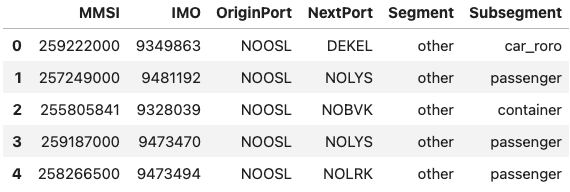
\includegraphics[width=.8\textwidth]{figures/apw/apw_dataset.png}
    \caption{A sample of the dataset used in the feasibility study}
    \label{fig:apw_dataset}
\end{figure}

In the feasibility study, there were two main steps in the analysis process. Firstly, a single-case analysis was conducted on a port known to the author to establish a more thorough overview of the traveling patterns of different vessel types and to gain an understanding of how to interpret the results. Secondly, a trend analysis was conducted on a collection of ports in order to establish a recurring pattern. In the study, a few major ports were selected combined with a few ports known to the author and experts in \acrshort{mo}. The complete list of ports are listed in \cref{sec:trend_analysis}.

\section{Single-case analysis}

For the single-case analysis, the port of Oslo (\texttt{NOOSL}) was selected as it is frequented by both dry bulk cargo vessels as well as several passenger vessels. It was presumed that the higher traveling frequency of the passenger vessels would heavily skew the most frequent next port for all vessels visiting \texttt{NOOSL}. Firstly, the distribution of the next frequented ports from the port was mapped as shown in \cref{fig:apw_noosl_freq} which shows that the port of Lysaker (\texttt{NOLYS}) is the most frequented next port by far. Lysaker port is a very small port that mostly receives passenger vessels that, as expected, would have high frequency because passenger vessels frequently travel back and forth over short distances. This also means that few passenger vessels could be responsible for almost all voyages, and predictions would be heavily skewed toward \texttt{NOLYS}.

\begin{figure}[htbp]
    \centering
    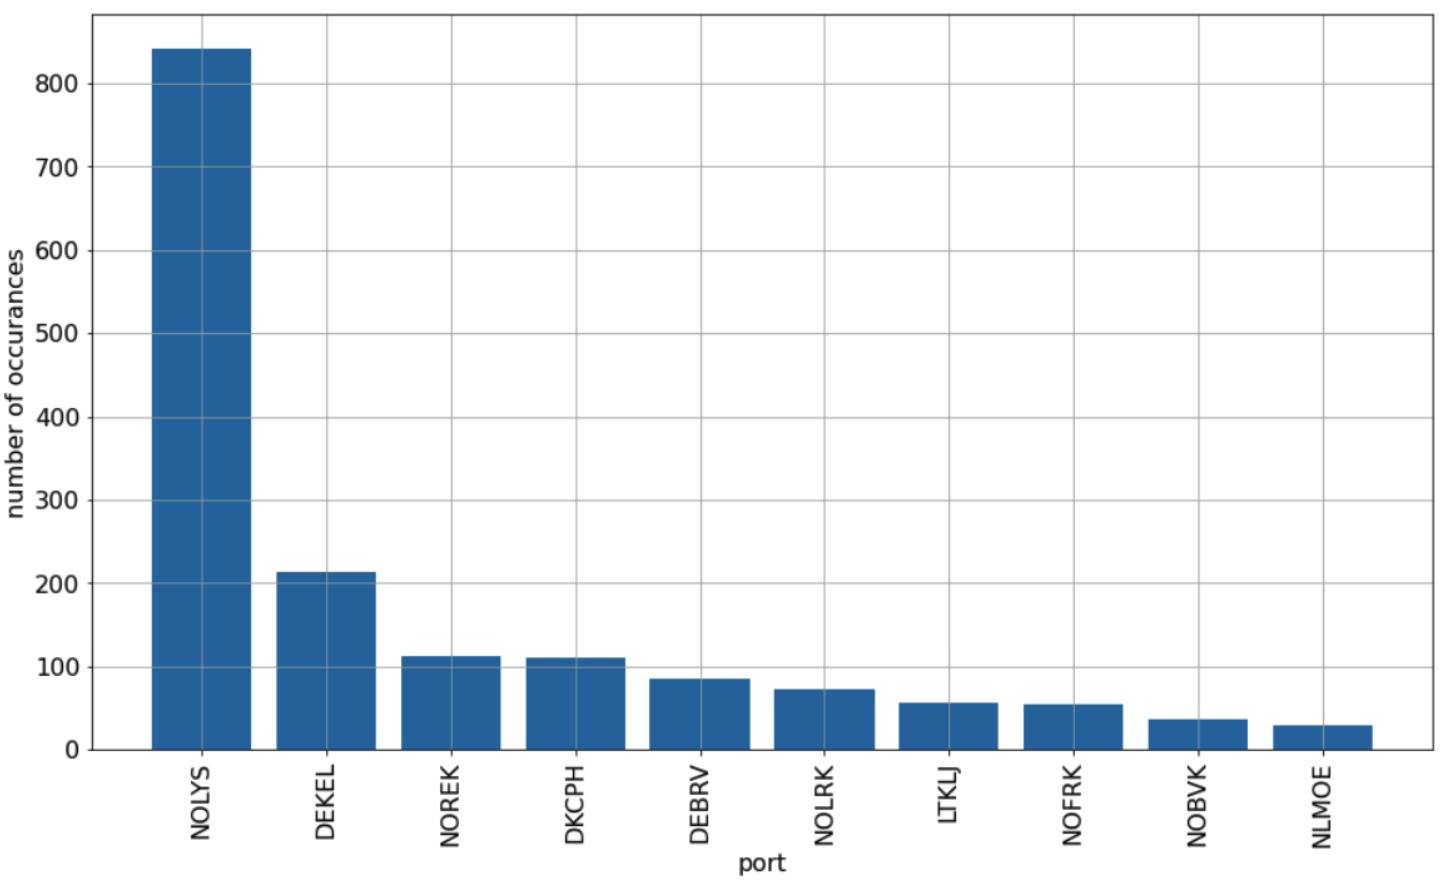
\includegraphics[width=.9\textwidth]{figures/apw/noosl_freq.png}
    \caption{Distribution of \textit{NextPort}s from \texttt{NOOSL}}
    \label{fig:apw_noosl_freq}
\end{figure}

When looking into the distributions of \textit{NextPort}s per segment it is even more apparent that the \textit{Other} segment (which includes passenger vessels) are responsible for the high number of voyages to \texttt{NOLYS}. \cref{fig:apw_noosl_segments} shows this as well as the \textit{Other} is the only segment that shares the same most frequent next port \texttt{NOLYS}. This means that a prediction algorithm using port frequencies would accurately predict the next destination ports for these other vessels, but not for the rest. Since the other vessels are responsible for 1568 out of 2009 transitions (78.05\%), considering vessel segmentation for predictions, and assuming every vessel always travel to its segment most frequent next port, a prediction algorithm could also become accurate for the remainder of the vessel segments which adds up to 21.95\% of all transition and probably most of the unique vessels. This is the basis used to estimate an improvement, or impact, factor for vessel segmentation on destination predictions.

\begin{figure}[htbp]
    \centering
    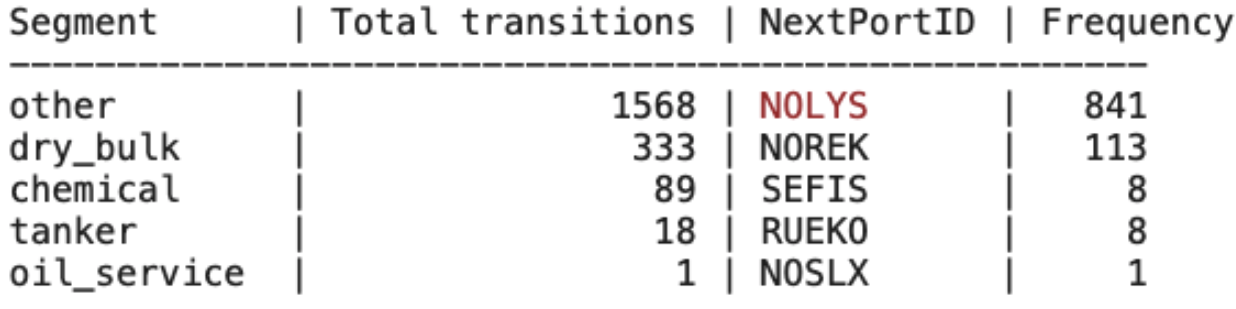
\includegraphics[width=.7\textwidth]{figures/apw/noosl_segments.png}
    \caption{Distribution of \textit{NextPort}s from \texttt{NOOSL} per segment}
    \label{fig:apw_noosl_segments}
\end{figure}

Furthermore, as \cref{fig:apw_noosl_dry_bulk} shows, when looking at the port frequency of the dry bulk cargo vessels, it is apparent that \texttt{NOLYS} is not even a contender for the most frequent next port. Therefore, a prediction method considering port frequencies would not be able to accurately predict the next destination port for any other vessel other than passenger vessels.

\begin{figure}[htbp]
    \centering
    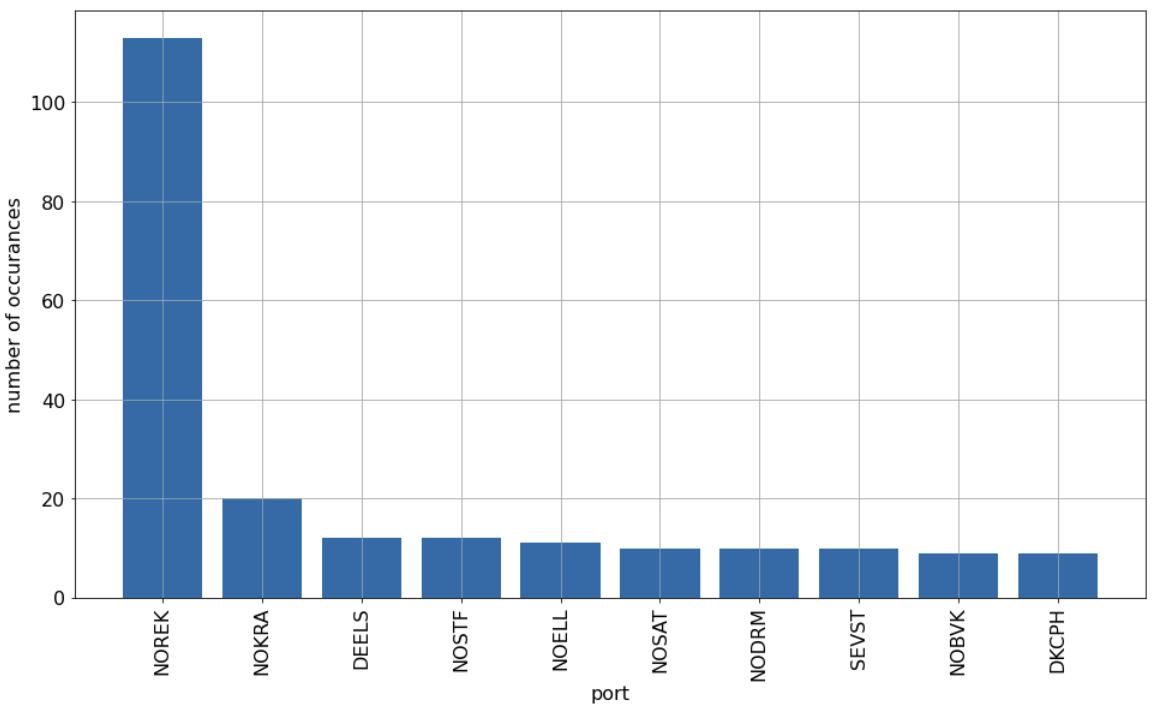
\includegraphics[width=.9\textwidth]{figures/apw/noosl_dry_bulk.png}
    \caption{Distribution of \textit{NextPort}s from \texttt{NOOSL} for the \textit{"dry bulk" segment}}
    \label{fig:apw_noosl_dry_bulk}
\end{figure}

Investigating sub-segments further confirms that a few numbers of vessels are responsible for most of all total transitions. \cref{fig:apw_noosl_subsegments} shows that the specific sub-segment \textit{other - passenger}, or passenger vessels, are responsible for 49.52\% of all transitions and nearly all voyages arrive at \texttt{NOLYS} after \texttt{NOOSL}. This means a prediction model could potentially be improved by 50\% if it would be aware of the sub-segment of each vessel for this particular port. \texttt{NOOSL} seems to be a port that shows the problem area quite well because it is a smaller port that receives a lower number of different vessels, and when there are multiple passenger vessels frequently arriving at it, they heavily skew the results in their favor.

\begin{figure}[htbp]
    \centering
    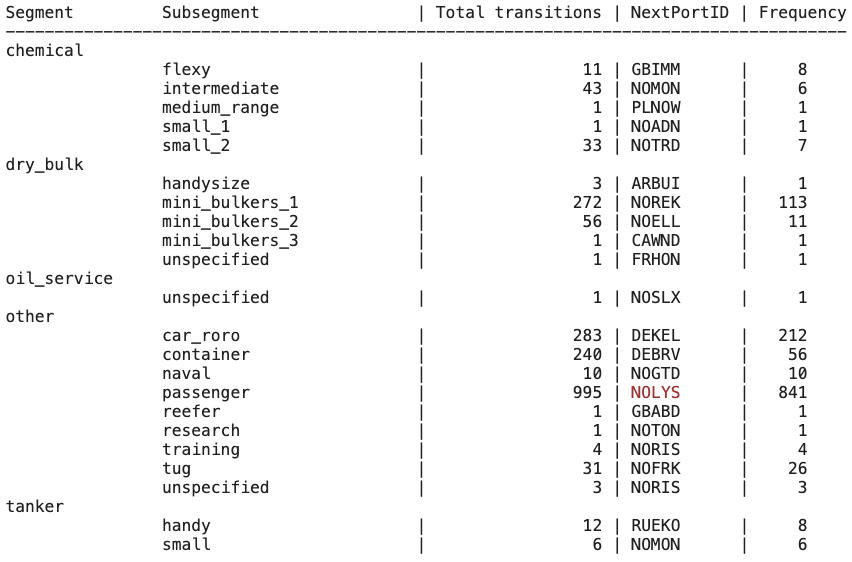
\includegraphics[width=.8\textwidth]{figures/apw/noosl_subsegments.png}
    \caption{Distribution of \textit{NextPort}s from \texttt{NOOSL} per sub-segment}
    \label{fig:apw_noosl_subsegments}
\end{figure}


\section{Trend analysis}
\label{sec:trend_analysis}

As already mentioned, for the trend analysis, a number of ports were selected based on their size and traffic. There were also a couple of known ports included in this dataset to easier interpret the results. The ports used in the analysis were:

\begin{itemize}
    \item \texttt{NLRTM} - Rotterdam, Netherlands
    \item \texttt{NOOSL} - Oslo, Norway
    \item \texttt{CNSHG} - Shanghai, China
    \item \texttt{NLMSV} - Maasvlakte, Netherlands
    \item \texttt{SGSIN} - Singapore, Singapore
    \item \texttt{USHPY} - Baytown, USA
    \item \texttt{BEANR} - Antwerpen, Belgium
    \item \texttt{TWKHH} - Kaohsiung, Taiwan
    \item \texttt{JPYOK} - Yokohama
\end{itemize}

The same process as for the single-case analysis was conducted, but on a higher level as the main purpose of this study was to establish a trend in terms of a impact factor of vessel segmentation on port frequencies. \cref{fig:trend_freq} shows a similar version of the table used for the single port analysis (\cref{fig:apw_noosl_freq}) but also shows the number of transitions that differed from the most frequent next port when considering segments (i.e. the estimated improvement factor).

\begin{figure}[htbp]
    \centering
    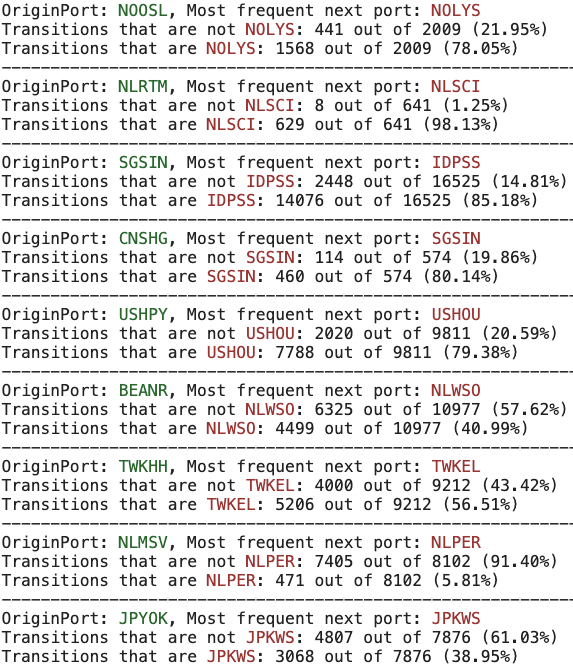
\includegraphics[width=.56\textwidth]{figures/apw/trend_frequency.png}
    \caption{Port frequencies and transition distribution as they relate to the most frequent next port for the selected ports}
    \label{fig:trend_freq}
\end{figure}

\begin{figure}[htbp]
    \centering
    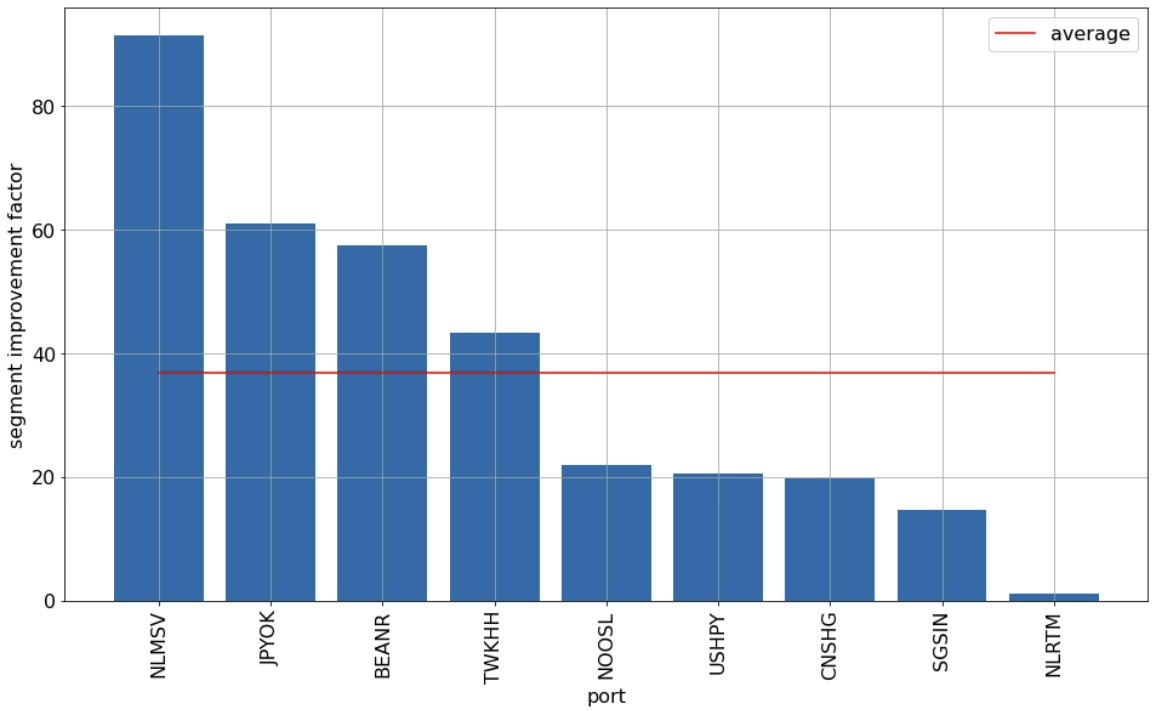
\includegraphics[width=.9\textwidth]{figures/apw/segment_improvement.png}
    \caption{Distribution of improvement factors for each origin port considering segments}
    \label{fig:segment_improvment}
\end{figure}

It is apparent that there are variances in improvement factors for different ports ranging from as low as \textit{1.25\%} to as high as \textit{91.40\%}. In the case of \texttt{NLRTM}, which is mostly a dry bulk port, there were no considerable improvements as almost all vessels are of the same segment. For the port \texttt{NLMSV}, the opposite was the case as there were a plethora of different types of vessels that frequented the port. \cref{fig:segment_improvment} shows the distribution of the improvement factor considering segments for each origin port as well as the overall average impact factor for these 9 ports which was \textit{36.88\%}.

Furthermore, when looking at the impact of sub-segments, as \cref{fig:subsegment_improvment} shows, it seems that the improvement factor has increased overall. For example, in the case of \texttt{NLRTM}, the improvement factor has increased from \textit{1.25\%} to \textit{19.66\%}, and although this varied for the different ports, the overall average improvement factor increased from \textit{36.88\%} to \textit{50.28\%}.

\begin{figure}[htbp]
    \centering
    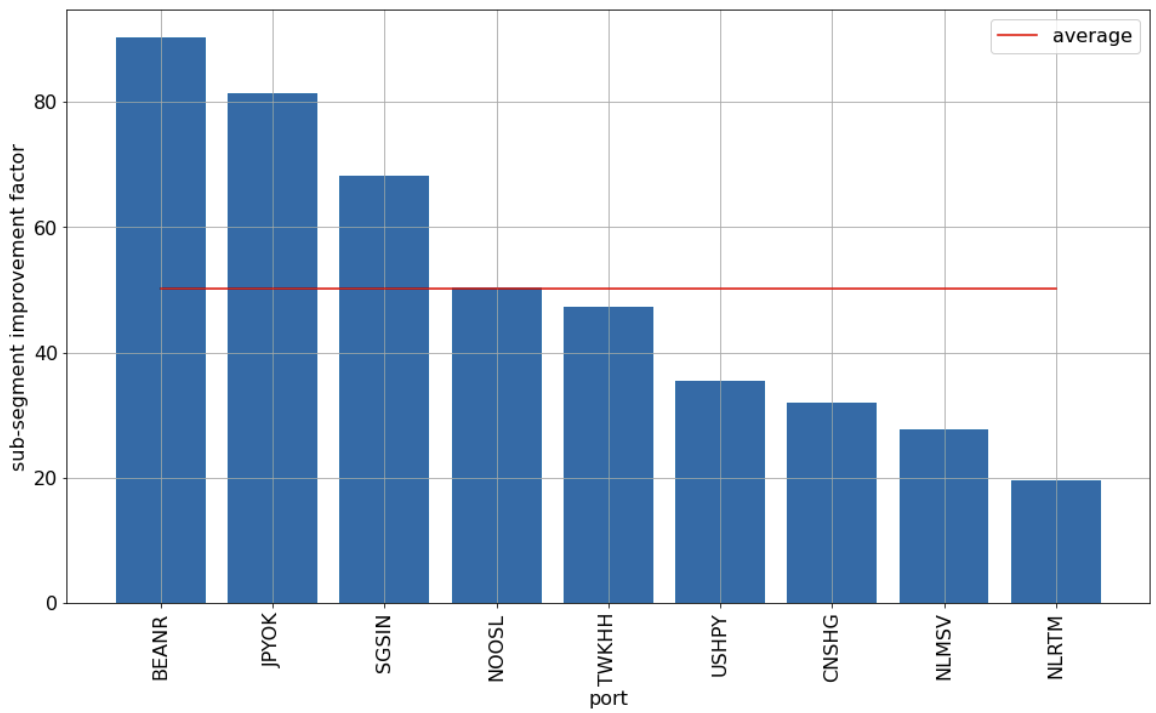
\includegraphics[width=.9\textwidth]{figures/apw/subsegment_improvement.png}
    \caption{Distribution of improvement factors for each origin port considering sub-segments}
    \label{fig:subsegment_improvment}
\end{figure}

A prediction method considering the frequencies of ports for vessel destination predictions would choose the most frequent next port for the predicted next destination. In this scenario, ignoring the vessel's type (segmentation) would give the wrong prediction for a lot of vessels from different segments in a lot of ports. The results from the feasibility study clearly indicates that applying the aspect of vessel segmentation to such models would definitively have an impact on prediction accuracy and, therefore, is worth investigating further. Moreover, assuming this impact would also, to some degree, apply to vessel trajectories as they relate to traveling patters, improving the accuracy of a model such as the one described in \cite{ZHANG2020102729} seems to be plausible depending on the data foundation.
\chapter{Methodology}

\section{Processed dataset used for analysis}

\subsection{Vessel position history}

\begin{itemize}
    \item Validated on geographical coordinates
    \item Validated on MMSI -> IMO mapping and valid values
    \item Filtered from 1 billion to 450 million etc...
    \item Visualization ?
\end{itemize}

\subsection{Vessel transitions}

 - A direct copy of MO's
 
 \subsection{Ports}
 
 - A direct copy of MO's "visible" ports
 
 \subsection{Segments}
 
 - A direct copy of MO's
 
 \subsection{Transition voyages}
 
 \subsection{Clustered voyages}
 

\chapter*{\bibname}
\printbibliography[heading=none]

% First paper

\begin{paper}{papers/landes1951scrutiny.pdf}{paper:scrutiny}
    Here, you may add a description of the paper, an illustration, or just give the bibliographic reference:
    \begin{quote}
        hello world
    \end{quote}
    Or you may leave it empty, if you like.
\end{paper}

% Second paper etc.

\appendix
\chapter{Additional Material}
\label{app:additional}

Additional material that does not fit in the main thesis but may still be relevant to share, e.g., raw data from experiments and surveys, code listings, additional plots, pre-project reports, project agreements, contracts, logs etc., can be put in appendices. Simply issue the command \texttt{\textbackslash appendix} in the main \texttt{.tex} file, and make one chapter per appendix.

If the appendix is in the form of a ready-made PDF file, it should be supported by a small descriptive text, and included using the \texttt{pdfpages} package. To illustrate how it works, a standard project agreement (for the IE faculty at NTNU in Gjøvik) is attached here. You would probably want the included PDF file to begin on an odd (right hand) page, which is achieved by using the \texttt{\textbackslash cleardoublepage} command immediately before the \texttt{\textbackslash includepdf[]\{\}} command. Use the option \texttt{[pages=-]} to include all pages of the PDF document, or, e.g., \texttt{[pages=2-4]} to include only the given page range.


\end{document}
